\chapter{Implementations}

\section{Development Environment}

Whatever client side or server side, there always framework depended, so build development environment is inevitable. In this project, the server is encoded using NodeJS. With limited space, for basic NodeJS environment, such as common configuration tool, NPM package management are omitted in this thesis. Here we introduce the most important framework structure and build of this platform, LeapJS; On client side, we use Swift to code and we do not import any third party framework, but WatchConnectivity need to be use for communication\cite{WatchConnectivity:2016}.
After iOS 9, every App in iOS need to use HTTPS request, but there is a way to configure HTTP request in iOS 9.
%无论是手表端的还是服务端,都存在框架依赖,因此环境搭建不可避免。在本项目中,服务端使用 NodeJS 进行编码,限于篇幅,对 NodeJS 相关的基本环境,如 Node 本体,NPM 包管理等常见工具的配置在文中略去,这里主要介绍运行本平台最重要第三方 Leap Motion 环境;而在手表端中,虽然我们不依赖其他第三方框架,但由于 watchOS 自身的限制\cite{WatchConnectivity:2016} 在 watchOS 2 中我们需要使用 WatchConnectivity 框架与 iOS 应用本体进行数据通信。
%由于 iOS 系统本身限制(iOS 9及以上)强制要求应用必须与 HTTPS 服务器进行通信,因此这里介绍在 iOS 9 中与 HTTP 服务器通信的配置方法。

\subsection{Configuration of Local LeapMotion}

LeapMotion provides development environment in Mac OS X, and provides a variety of programming language. Based on above discussion, we need to configure the server LeapMotion body and LeapJS.
%LeapMotion 提供了在 Mac OS X 中的开发环境,并且提供了各种不同的开发语言,根据上文的讨论,我们需要在服务端配置 LeapMotion 本体以及 LeapJS。

\textbf{1. Installation}

First of all, to use LeapMotion API, we have to import LeapSDK into our desktop host application.
%首先,在应用程序中引入 Leap SDK 需要在相应桌面端安装 LeapMotion 宿主程序,进而才能使用 LeapMotion 相关的 API。

Secondly, we need add dependency of LeapJS in Node App's package.json file:
%其次,在 Node App 的 package.json 中添加 LeapJS 依赖:
\begin{lstlisting}[frame=trBL,frameround=fttt,rulesepcolor=\color{white},numbers=none]
"dependencies": {
    "leapjs": "^0.6.4"
}
\end{lstlisting}

The next step is install LeapJS by npm install.
%再使用 npm install 安装 LeapJS。

\textbf{2. Configs}

By the limitations of LeapMotion\cite{Leap:2016}, WebSocket service doesn't open a non-local access in default setting, so we will need to configure Leap then enable non-local client connections.
%受到 LeapMotion 自身的限制\cite{Leap:2016},WebSocket 服务并非默认的向非本地访问开放,因此需要将 Leap 配置启用非本地客户端连接。

This requires to configure LeapMotion profile. Before we modify the configuration, we have to close LeapMotion related services. On Mac OS X, we use the following command to shut down LeapMotion daemon:
%这需要对 LeapMotion 的配置文件进行修改。在修改配置之前,需要关闭 LeapMotion 的相关服务。在 Mac 中,使用下面的命令关闭 LeapMotion 的守护进程:

\begin{lstlisting}[frame=trBL,frameround=fttt,rulesepcolor=\color{white},numbers=none]
sudo launchctl unload /Library/LaunchDaemons/com.leapmotion.leapd.plist
\end{lstlisting}

Next, we need to modify LeapMotion profile. According to the official documents , Leap contains two different configurations and the highest priority belongs to control panel, so we need edit the following directory:
%接下来我们需要修改 LeapMotion 的配置文件,根据 LeapMotion 的官方文档显示,Leap 包含两个不同的配置,其中控制面板配置的优先级最高,因此我们需要下面这个目录下:

\begin{lstlisting}[frame=trBL,frameround=fttt,rulesepcolor=\color{white},numbers=none]
$HOME/Library/Application\ Support/Leap\ Motion
\end{lstlisting}

Find config.json configuration file, editing config.json file and add an arbitrary position in the configuration field:
%找到 config.json 的修改配置,编辑 config.json 文件,并在 configuration 字段中的任意位置添加一条:

\begin{lstlisting}[frame=trBL,frameround=fttt,rulesepcolor=\color{white},numbers=none]
"websockets_allow_remote": true
\end{lstlisting}

%最终得到:
finally obtained:

\begin{lstlisting}[frame=trBL,frameround=fttt,rulesepcolor=\color{white},numbers=none]
"configuration": {
    "websockets_allow_remote": true,
    "background_app_mode": 2,
    "images_mode": 2,
    "interaction_box_auto": true,
    "power_saving_adapter": true,
    "robust_mode_enabled": false,
    "tracking_tool_enabled": true
}
\end{lstlisting}

%保存退出,重新启动 LeapMotion 服务,便完成了 LeapMotion 的相关配置:
save and quit, restart LeapMotion Service and then we finished the configuration of LeapMotion:

\begin{lstlisting}[frame=trBL,frameround=fttt,rulesepcolor=\color{white},numbers=none]
sudo launchctl load /Library/LaunchDaemons/com.leapmotion.leapd.plist
\end{lstlisting}

\subsection{watchOS Networking Access}

From iOS 9. Apple introduced App Transport Security feature for iOS App, this causes iOS App could not access to the Interaction with HTTP requests.
%从 iOS 9 开始, iOS 对网络访问引入了 App Transport Security (ATS) 特性,这使得在默认状态下 iOS 应用无法发起非安全的网络请求(如 HTTP)。

Due to watchOS networking need iOS App to transfer its requests in the most of time, we need applying two more configuration steps, and the results shows on Figure \ref{fig:config}.
%需要进行下列两个步骤配置项目,结果如图\ref{fig:config}所示:

\begin{enumerate}
    \item Add NSAppTransportSecurity as a Dictionary type into Info.plist;
    %在Info.plist中添加NSAppTransportSecurity类型Dictionary;
    \item Add NSAllowsArbitraryLoads key as a Boolean type into NSAppTransportSecurity, then set its value YES.
    %在NSAppTransportSecurity下添加NSAllowsArbitraryLoads类型Boolean,值设为YES
\end{enumerate}

\begin{figure}[H]
    \kaishu
    \centering
    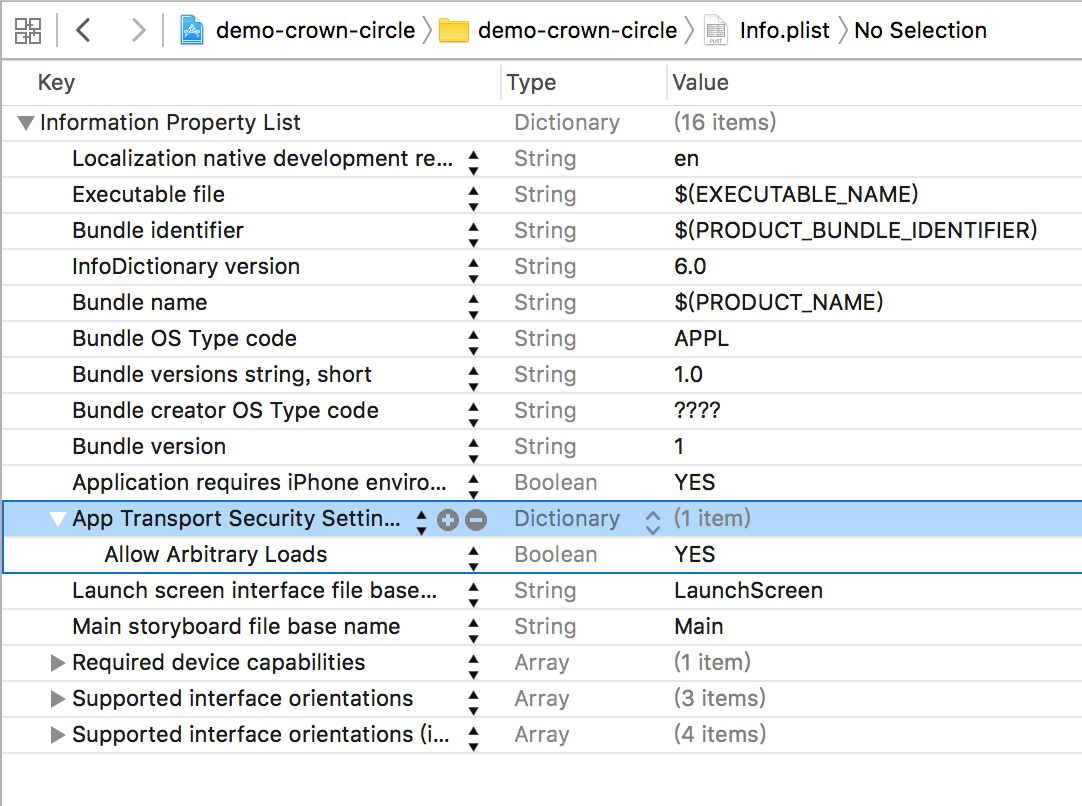
\includegraphics[width=0.4\textwidth]{figures/config}
    \caption{\kaishu Configuration results of info.plist file} %配置客户端 info.plist 文件}
    \label{fig:config}
\end{figure}

\section{Server Side}
To archive a HTTP Server with port 10086 is the first step of developing, it is implement by NodeJS and codes shows on Code \ref{lst:http}.
%实现一个端口为 10086 的 HTTP 服务器是第一步,如代码\ref{lst:http}。
\begin{lstlisting}[
    language={JavaScript},
    caption={\kaishu Create HTTP server on 10086},
    label={lst:http}
]
var http = require('http');
function handler (req, res) {
    res.writeHead(200);
}
http.createServer(handler).listen(10086);
console.log("Server running at http://locoalhost:10086")
\end{lstlisting}

Now, we focus on how to process LeapMotion Gesture in the following content.
%下面我们来关注服务端中对 LeapMotion 手势的关键处理。

\subsection{Tap and Force Touch Processing}

LeapMotion Software itself will reconstruct hand model of users, and its APIs provide the skeleton data, including fingers tip position.
To recognize pinch gesture, we can calculate two finger tips, so that we can iterate all finger tips except thumb, the implementation code shows on Code \ref{lst:pincher}.
%LeapMotion 软件本身会对所识别手部进行重新建模,并提供其骨骼模型的全部数据,因此也包括对手指位置。
%而对于手指捏合的识别,可以转化为对两只手指指尖位置的判断,故可对除拇指外的其他四根手指中进行遍历,如代码\ref{lst:pincher} 所示。

\begin{lstlisting}[
    language={JavaScript},
    caption={\kaishu Tap Gesture Recognize},
    label={lst:pincher}
]
function findPinchingFinger(hand, closest){
    var pincher;
    //var closest = 500;
    for(var f = 1; f < 5; f++)
    {
        current = hand.fingers[f];
        distance = leap.vec3.distance(hand.thumb.tipPosition, current.tipPosition);
        if(current != hand.thumb && distance < closest)
        {
            closest = distance;
            pincher = current;
        }
    }
    // mark time of start pinch
    if (pincher.type != pf.pinchIndex) {
        // pf is a gloable value for message protocol
        pf.pinchTimeStramp = Date.now();
    }
    return pincher;
}
\end{lstlisting}

We have discussed Force Touch simulation in Subsection \ref{sub:force-touch-simu}, now the implementation of JavaScript code shows on Code \ref{lst:ft-simu}.
%对于 Force Touch 的模拟在\ref{sub:force-touch-simu}一节中已经详细描述过方法,其核心实现如代码\ref{lst:ft-simu}所示。

\begin{lstlisting}[
    language={JavaScript},
    caption={\kaishu Force Touch Simulation},
    label={lst:ft-simu}
]
function forceValue(){
    // pf is the global message protocol object
    if (pf.pinchTimeStramp === 0) {
        return -1;
    }

    var delay = 250;
    var duration = 1000;

    // calculate force touch value
    var value = ((Date.now() - pf.pinchTimeStramp) - delay)/duration;
    var force = (value >=1 ) ? 1 : value*value;

    return force;
}
\end{lstlisting}

\subsection{Two Fingers Swipe}

For two fingers swipe, it seems difficult to identify, but in fact we can converted it to pinch degree between two fingers.
In fact LeapMotion itself provides thumb and index finger pinch degree parameter, but because of its results is universe for every fingers and cannot customize by developer. For this reason, we have to reimplement this function.
%对于双指之间滑动的识别看似困难,但实际上我们可以将其转化为两指之间的捏合度。其实 LeapMotion 本身提供了对拇指和食指捏合度参数,但由于其结果为一般情况下的捏合度,即在任何收拾下都存在捏合度,而对于我们来说需要控制交互,构建双指滑动的触发事件,因此我们有必要重新实现这个功能。

\begin{figure}[H]
\kaishu
\centering
\subfigure[Before]{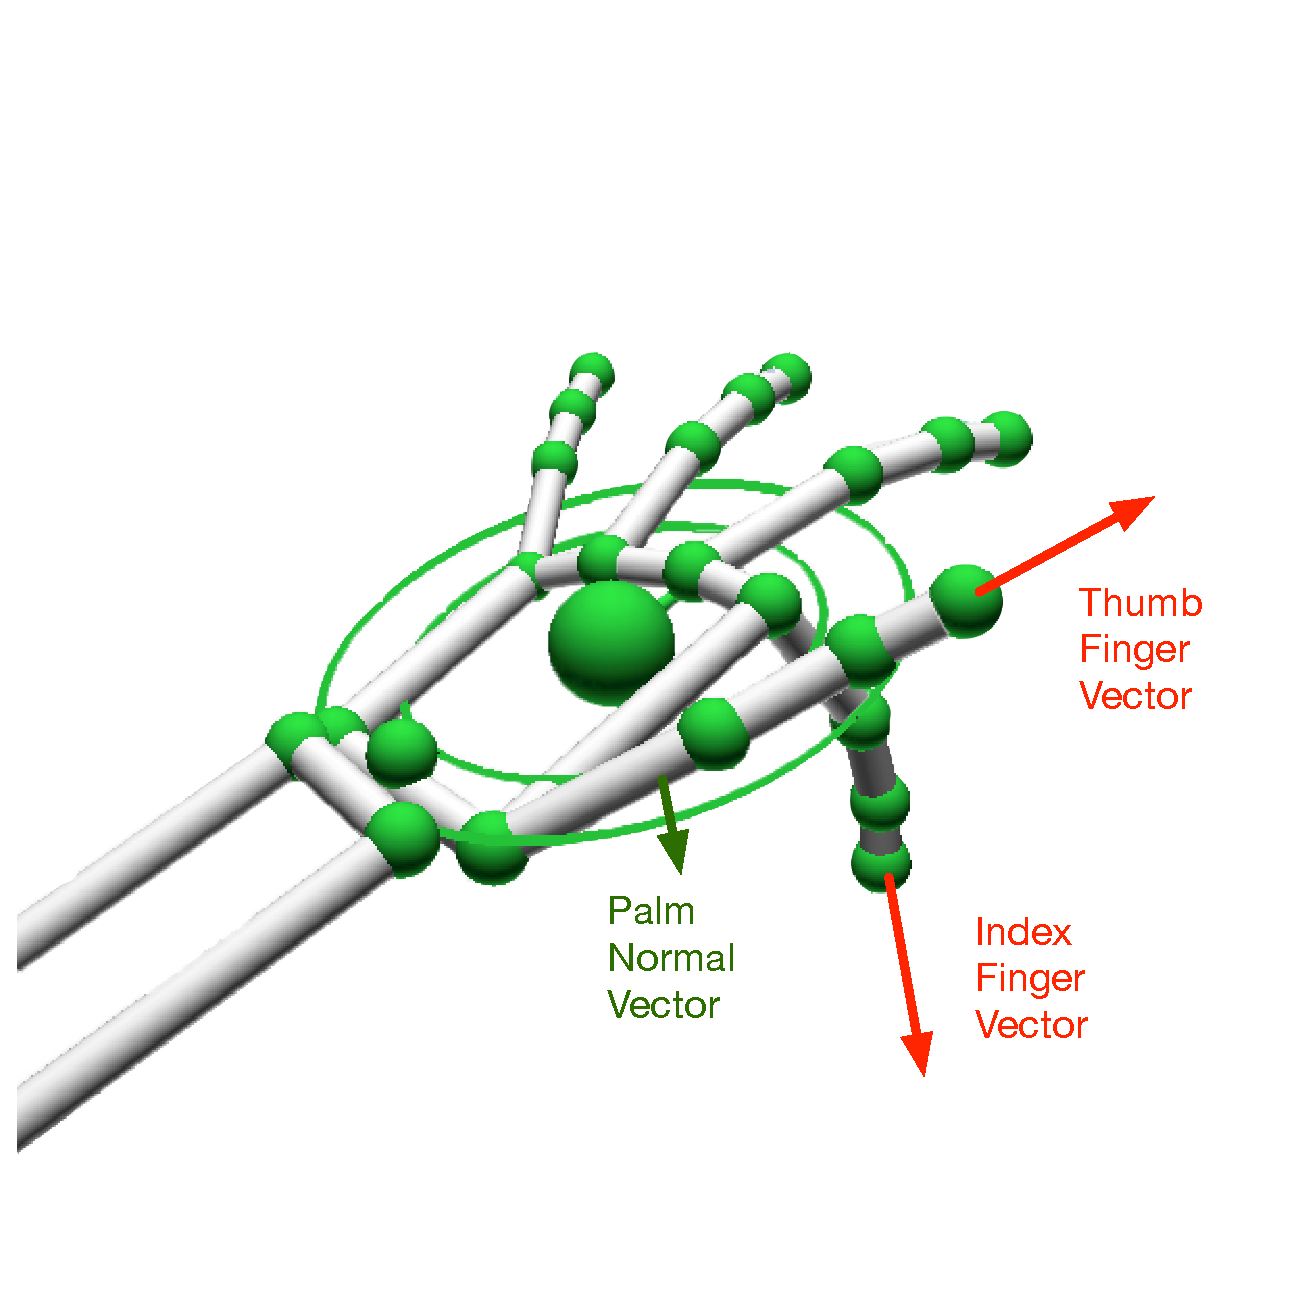
\includegraphics[width=0.35\textwidth]{figures/pinch-start}\label{fig:pinch-start}}
\subfigure[After]{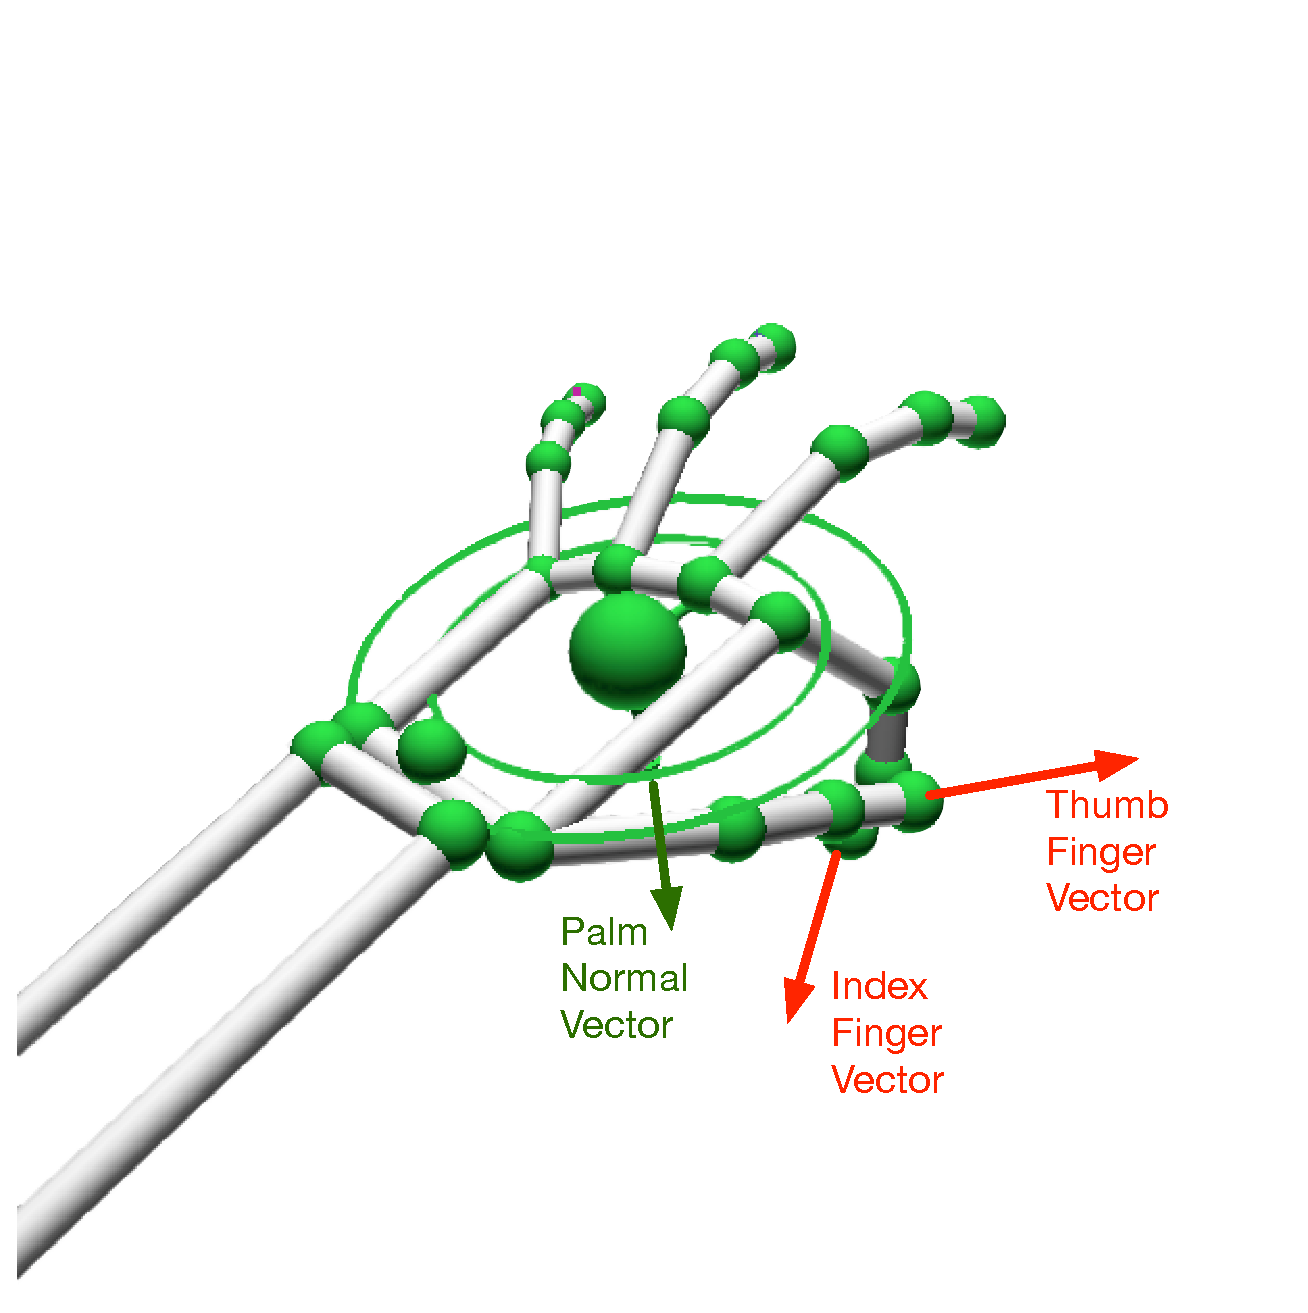
\includegraphics[width=0.35\textwidth]{figures/pinch-end}\label{fig:pinch-end}}
\caption{\textbf{Two finger swipe}: two finger swipe can trigger events by palm normal vector and finger direction vector, 3D models in this figure are generate by LeapMotion Visualizer}
\label{fig:pinch}
\end{figure}


Two finger swipe gesture shows on Figure \ref{fig:pinch}, when hand  presented as Figure \ref{fig:pinch-start}, the normal vector of palm and direction vector of index infer are parallel, thumb direction vector and palm normal vector are almost vertical, so we can use this character to trigger this events, as its illustrate on Code \ref{lst:swipe}.
%双指滑动手势如图\ref{fig:pinch}所示,当手呈现如图\ref{fig: pinch-start}所示手势时,食指的方向向量和手掌的法向量几乎平行,拇指的方向向量与手掌的法向量几乎垂直,故我们可以利用这个特点设计手势的触发事件。如代码\ref{lst:swipe}:

\begin{lstlisting}[
    language={JavaScript},
    caption={\kaishu Two fingers swipe recognize},
    label={lst:swipe}
]
function findPinchingStrength(hand) {
    var thumbDirection = hand.fingers[0].direction;
    var indexDirection = hand.fingers[1].direction;
    var dotProduct = leap.vec3.dot(thumbDirection, indexDirection);
    // remove grab condition
    if (dotProduct < 0.7 && hand.grabStrength < 0.85) {
        return hand.pinchStrength;
    } else {
        return -1;
    }
}
\end{lstlisting}

\subsection{Grab}

We don't need reimplement grab gesture, LeapMotion itself provides grab parameter of a hand, we can straightly get this data from Frame object, as shown on Code \ref{lst:grab}.
%五指的合并不需要重新实现,LeapMotion 本身就提供了握拳程度的参数 grabStrength,我们可以直接从 Frame 对象中获取,如代码\ref{lst:grab}所示。

\begin{lstlisting}[
    language={JavaScript},
    caption={\kaishu grab recognize},
    label={lst:grab}
]
grabStrength = function getGrabStength(frame) {
    return frame.hands[0].grabStrength;
}
\end{lstlisting}

\section{Client Side}

The key of client encoding is the communication layer and view controller layer , communication layer also contains communications between iOS, watchOS and server, we use Swift \footnote{Swift version 2.2.} to complete the associated code \cite{swift2015, swiftoc2015}.
%客户端编码的两个重要关键就是通信层和视图控制层的编码,通信层又包含 iOS 端和服务端之间通信以及 iOS 端和 watchOS 端间通信,我们使用 Swift \footnote{本文写成时的 Swift 版本为 2.2。}来完成相关编码\cite{swift2015, swiftoc2015}。

\subsection{View Controller Layer}

View Controller Layer is basically a response for interactive message, as an example, we shows the core code of design for two finger swipe gesture as a Digital Crown alternative design.
%视图控制层是对交互消息本身的一个响应,这里的代码以双指滑动的 Digital Crown 表达为例,展示核心设计。

Picker class on Apple Watch need developer load resources themselves, code as shown on Code \ref{lst:picker}.
%在 Apple Watch 上实现 Picker 需要应用开发者自行加载相关资源,其代码段如代码\ref{lst:picker}所示。

\begin{lstlisting}[
    language={Swift},
    caption={\kaishu Load resources of Picker class},
    label={lst:picker}
]
var images: [UIImage]! = []
var pickerItems: [WKPickerItem]! = []
for (var i=0; i<=MAX_NUM; i += 1) {
    let name = "progress-\(i)"
    images.append(UIImage(named: name)!)

    let pickerItem = WKPickerItem()
    pickerItem.title = "\(i)"
    pickerItems.append(pickerItem)
}
let circleImages = UIImage.animatedImageWithImages(images, duration: 0.0)
circleGroup.setBackgroundImage(circleImages)
picker.setCoordinatedAnimations([circleGroup])
picker.setItems(pickerItems)
\end{lstlisting}

We mapping the pinchStrength value from [0,1] to [0, MAX\_NUM], then use setter function of Picker to modify UI interface, as shown on Code \ref{lst:ui-op}.
%而对于 Digital Crown 的表达,则是在通过网络层接收到交互信息 pinchStrength 后,将 0 至 1 的数值变换到 Picker 所拥有的 0 至 MAX\_NUM,然后通过设置 Picker 的选择项来操纵 UI 界面,如代码\ref{lst:ui-op}所示。

\begin{lstlisting}[
    language={Swift},
    caption={\kaishu Picker UI manipulate},
    label={lst:ui-op}
]
func indexSelect(message: InteractionMessage?) {
    index = Int(message!.pinchStrength * MAX_NUM)
    // haptic feedback
    watchDevice.playHaptic(WKHapticType.DirectionUp)
    picker.setSelectedItemIndex(index)
}
\end{lstlisting}

\subsection{Communication Layer}

To communicate with the server, we can use HTTP request from server to gesture data, which is in JSON format. In Code \ref{lst:connectserver}, completeFlag guarantees only after a previous request completes program will trigger next request out. The constructor of Gesture class will parsing JSON data and contract a Gesture object model from the data dictionary.
%与服务端的通信通过 URL 请求服务端的手势数据,其结果为 JSON 格式数据。在代码\ref{lst:connectserver}中, completeFlag 保证了向服务器请求对象时仅在上一次请求完成后才能进行,而 Gesture 类的构造函数通过从 URL 中解析来的 JSON 数据字典构造 Gesture 对象模型。

\begin{lstlisting}[
    language={Swift},
    caption={\kaishu Communication between iOS and Server},
    label={lst:connectserver}
]
func connectServer() {
    // member variable
    if completeFlag == 0 {
        return
    }
    task = session.dataTaskWithURL(url, completionHandler: { (data, res, error) -> Void in
        if let e = error {
            print("dataTaskWithURL fail: \(e.debugDescription)")
            return
        }
        if let d = data {
            print("\(NSString(data: d, encoding: NSUTF8StringEncoding))")

            if let jsonObj = try? NSJSONSerialization.JSONObjectWithData(d, options: NSJSONReadingOptions.AllowFragments) as? NSDictionary {
               self.Gesture = Gesture(fromDictionary: jsonObj!)
            }
            self.completeFlag = 1

        }
    })
    task!.resume()
}
\end{lstlisting}

To establish a connection between iOS and watchOS, the only way to archive this is to use WatchConnectivity framework, Code \ref{lst:ios-watchos} and Code \ref{lst:watchos-ios} list the core implementation of send message to watchOS and receive message from iOS.
%在 iOS 端和 watchOS 端之间通信需要利用 WatchConnectivity 框架,代码包含 iOS 端发送以及 watchOS 端接受,如代码\ref{lst:ios-watchos} 和 \ref{lst:watchos-ios}所示。

\begin{lstlisting}[
    language={Swift},
    caption={\kaishu \textbf{Communication between iOS and watchOS}: Send Message},
    label={lst:ios-watchos}
]
func updateMessage() {
    if WCSession.defaultSession().reachable {
        let content:[String:String] = ["x":PinchFinger.text!, "y":PinchStrength.text!, "z":GrabStrength.text!]
        let message = ["up": content]
        WCSession.defaultSession().sendMessage(
            message, replyHandler: { (replyMessage) -> Void in
                print("send success..")
            }) { (error) -> Void in
                print(error)
        }
    }
}
\end{lstlisting}
\begin{lstlisting}[
    language={Swift},
    caption={\kaishu \textbf{Communication between watchOS and iOS}: Receive message},
    label={lst:watchos-ios}
]
extension InterfaceController: WCSessionDelegate {
    func session(session: WCSession, didReceiveMessage message: [String : AnyObject]) {
        guard message["up"] as? [String:String] != nil else {return}
        let contents = message["up"] as! [String : String]
        self.interaction(contents)
    }
}
\end{lstlisting}

\cleardoublepage
